\documentclass[preprint, 3p,
authoryear]{elsarticle} %review=doublespace preprint=single 5p=2 column
%%% Begin My package additions %%%%%%%%%%%%%%%%%%%

\usepackage[hyphens]{url}

  \journal{Transport Geography?} % Sets Journal name

\usepackage{graphicx}
%%%%%%%%%%%%%%%% end my additions to header

\usepackage[T1]{fontenc}
\usepackage{lmodern}
\usepackage{amssymb,amsmath}
% TODO: Currently lineno needs to be loaded after amsmath because of conflict
% https://github.com/latex-lineno/lineno/issues/5
\usepackage{lineno} % add
\usepackage{ifxetex,ifluatex}
\usepackage{fixltx2e} % provides \textsubscript
% use upquote if available, for straight quotes in verbatim environments
\IfFileExists{upquote.sty}{\usepackage{upquote}}{}
\ifnum 0\ifxetex 1\fi\ifluatex 1\fi=0 % if pdftex
  \usepackage[utf8]{inputenc}
\else % if luatex or xelatex
  \usepackage{fontspec}
  \ifxetex
    \usepackage{xltxtra,xunicode}
  \fi
  \defaultfontfeatures{Mapping=tex-text,Scale=MatchLowercase}
  \newcommand{\euro}{€}
\fi
% use microtype if available
\IfFileExists{microtype.sty}{\usepackage{microtype}}{}
\usepackage[]{natbib}
\bibliographystyle{plainnat}

\usepackage{graphicx}
\ifxetex
  \usepackage[setpagesize=false, % page size defined by xetex
              unicode=false, % unicode breaks when used with xetex
              xetex]{hyperref}
\else
  \usepackage[unicode=true]{hyperref}
\fi
\hypersetup{breaklinks=true,
            bookmarks=true,
            pdfauthor={},
            pdftitle={Leveraging GTFS to explore spatial gaps in transit supply with respect to social needs},
            colorlinks=false,
            urlcolor=blue,
            linkcolor=magenta,
            pdfborder={0 0 0}}

\setcounter{secnumdepth}{5}
% Pandoc toggle for numbering sections (defaults to be off)


% tightlist command for lists without linebreak
\providecommand{\tightlist}{%
  \setlength{\itemsep}{0pt}\setlength{\parskip}{0pt}}

% From pandoc table feature
\usepackage{longtable,booktabs,array}
\usepackage{calc} % for calculating minipage widths
% Correct order of tables after \paragraph or \subparagraph
\usepackage{etoolbox}
\makeatletter
\patchcmd\longtable{\par}{\if@noskipsec\mbox{}\fi\par}{}{}
\makeatother
% Allow footnotes in longtable head/foot
\IfFileExists{footnotehyper.sty}{\usepackage{footnotehyper}}{\usepackage{footnote}}
\makesavenoteenv{longtable}



\usepackage{subfig}
\usepackage{booktabs}
\usepackage{longtable}
\usepackage{array}
\usepackage{multirow}
\usepackage{wrapfig}
\usepackage{float}
\usepackage{colortbl}
\usepackage{pdflscape}
\usepackage{tabu}
\usepackage{threeparttable}
\usepackage{threeparttablex}
\usepackage[normalem]{ulem}
\usepackage{makecell}
\usepackage{xcolor}



\begin{document}


\begin{frontmatter}

  \title{Leveraging GTFS to explore spatial gaps in transit supply with
respect to social needs}
    \author[Public Transport Research Group (PTRG)]{James Reynolds%
  %
  \fnref{1}}
   \ead{james.reynolds@monash.edu} 
    \author[Public Transport Research Group (PTRG)]{Graham Currie%
  \corref{cor1}%
  \fnref{2}}
   \ead{graham.currie@monash.edu} 
    \author[Public Transport Research Group (PTRG)]{Yanda Qu%
  %
  \fnref{3}}
   \ead{yanda.qu@monash.edu} 
      \affiliation[Public Transport Research Group (PTRG)]{
    organization={Public Transport Research Group (PTRG), Institute of
Transport Studies, Department of Civil Engineering Engineering, Monash
University},addressline={Clayton
Campus},city={Melbourne},postcode={3800},state={Victoria},country={Australia},}
    \cortext[cor1]{Corresponding author}
    \fntext[1]{Research Fellow}
    \fntext[2]{Professor}
    \fntext[3]{PhD Student}
  
  \begin{abstract}
  This is the abstract.

  It consists of two paragraphs.
  \end{abstract}
    \begin{keyword}
    keyword1 \sep 
    keyword2
  \end{keyword}
  
 \end{frontmatter}

\hypertarget{introduction}{%
\section{Introduction}\label{introduction}}

A need to provide at least some motorised mobility for those who cannot
otherwise drive themselves influences transit service levels in many
places \citep{Currie:2016aa}. Age, disability, socio-economic status,
lack of a driver's license or vehicle, and many other factors might make
someone reliant on transit services for some or all of their travel.
Social-equity perspectives on transport policy-making, especially those
seeking to improve vertical equity so as to better support those who are
disadvantaged (c.f. \citet{Litman:2016aa}), might therefore suggest
providing at least some transit, and probably more than just a minimum,
to places that have the highest social need for transport. Previous
search developed an approach for identifying spatial gaps in transit
supply related to social needs for transport, which was applied to
Melbourne in 2006 \citep{Currie2007Identifying, currie2010identifying}.
However, there does not appear to have been much further use or
development of this approach. It is unclear whether the spatial patterns
identified in this previous research, are representative of transit
supply and social needs in other places, or whether the situation in
Melbourne has changed in the intervening years. This may in part be
because until recently transit schedule data was not readily available
in consistent, electronic formats, meaning that assessing transit supply
was a large task.

Nowadays, more than 10,000 transit agencies publicly release timetable
data in the General Transit Feed Specification (GTFS) format
\citep{GTFS}. Such standardisation allows Google Maps and other online
platforms to provide transit-related outputs for any place with a GTFS
feed, and has facilitated research and other analysis of transit
services. However, tools for using GTFS data to examine spatial patterns
and gaps in transit supply with respect to social needs for transport do
not appear to be readily available. This gap, and the lack of direct
follow up to \citet{Currie2003Hobart}, \citet{Currie2004Gap},
\citet{Currie2007Identifying} and \citet{currie2010identifying}, provide
the motivation for this paper.

The objectives of this research are: (1) to develop tools for
undertaking needs-gap analysis using GTFS datasets; and (2) to explore
whether the spatial pattern of gaps reported in
\citet{Currie2007Identifying} and \citet{currie2010identifying} are
consistent with current patterns; Research outcomes that are reported in
this paper include the development of a new R package (gtfssupplyindex)
with software tools that facilitate the \citet{Currie2007Identifying}
and \citet{currie2010identifying} approach, in particular the
calculation of transit Supply Index (SI) scores from GTFS datasets. Also
presented in this paper are results for Melbourne in 2016 and 2021,
matching the most recent censuses, which are compared across locations
and to the 2006 analysis reported in
\citet{currie2010identifying}\footnote{The wider programme of research
  includes examination of spatial gaps in other cities, so as to better
  understand whether patterns in Melbourne are representative of other
  places. However, this paper is limited to examining Melbourne only,
  and results for other cities will be reported elsewhere.}.

The remainder of this paper is structured as follows: the next section
outlines the background to this research. Section 3 describes the study
methodology, followed by presentation of results in Section 4 and
discussion in Section 5. Limitations of this study, directions for
future research and a brief conclusion are provided in Section 6.

\hypertarget{research-context}{%
\section{Research context}\label{research-context}}

\hypertarget{transit-metrics}{%
\subsection{Transit metrics}\label{transit-metrics}}

There are many metrics available for benchmarking transit services, with
examples including: those in the Transit Cooperative Research Program
(TCRP) Report 88 (a guidebook for developing performance-measurement
systems \citep{Ryus:2003aa}; and those used across benchmarking
databases and programs such as by
\citet{Florida-Transit-Information-System:2018aa}, the
\citet{UITP:2015aa} and \citet{Imperial-College-London:2023aa}. The
Fielding Triangle \citep{FieldingGordonJ1987Mpts} provides a framework
for combining indicators of service inputs, outputs and consumption to
describe cost efficiency, cost effectiveness and service effectiveness.
More broadly: \citet{Litman:2003ab} and \citet{Litman:2016aa} discuss
some of the traffic, mobility, accessibility, social equity, strategic
planning and other rational decision-making-based perspectives
underlying many transport indicators; \citet{Reynolds:2017ah} extends
these into models of how institutionalism, incrementalism and other
public policy analysis concepts might apply to decision-making processes
relating to transit prioritization; \citet{GuzmanLuisA.2017Aeit}
developed a measure of accessibility in the context of policy
development and social equity for Latin American Bus Rapid Transit (BRT)
networks; and \citet{Creutzig2020streetspaceallocation} introduced
street space allocation metrics based around ten ethical principles.

Many such metrics, however, may be difficult to calculate, explain or
understand, especially for those who are not planners, engineers or
other technical specialists. Where pre-calculated transit metrics are
immediately available, such as on a website or other online platform, it
may not be possible to independently generate scores, for instance to
assess proposed system changes. Contrasting examples are provided by:

\begin{itemize}
\item
  Transit Scores \citep{WalkScore:2023tg}, which are readily available
  online for locations with a published GTFS feed. The meaning of the
  metric appears easy to explain, with the highest possible score of 100
  representing the sort of transit accessibility experienced in the
  center of New York. However, the Transit Score algorithm is secret,
  and scores cannot be calculated independently or generated for
  proposed changes to a network.
\item
  The Transit Capacity and Quality of Service Manual (TCQSM), which
  provides a wide range of metrics for measuring different aspects of a
  transit system. The TCQSM scores themselves appear easy to understand
  or explain, ranging from A (good) to F (bad), although there are a
  large number of metrics. Scores, however, can be calculated
  independently, given sufficient data.
\end{itemize}

The widespread availability of GTFS datasets in recent years has
facilitated the development of tools that apply the same metric to many
transit systems. The Transit Score website provides one example.
\citet{Wong:2013aa} provides another in reporting the distribution of
various TCQSM metrics across 50 USA transit operators. Code used in the
\citet{Wong:2013aa} analysis is available for those who might wish to
produce a similar study for other locations and systems. Developing a
similar code base, but for calculating metrics associated with spatial
gaps in transit supply based on social needs, is the subject of this
paper.

\hypertarget{the-transit-suppy-index}{%
\subsection{The Transit Suppy Index}\label{the-transit-suppy-index}}

A generalized form of the SI equation, adapted from
\citet{currie2010identifying}, is:

\[SI_{area, time} = \sum{\frac{Area_{Bn}}{Area_{area}}SL_{n, time}}\]

where:

\begin{itemize}
\item
  \(SI_{area, time}\) is the Supply Index for the area of interest and a
  given period of time;
\item
  \(Area_{Bn}\) is the buffer area for each stop (n) within the area of
  interest (in \citet{currie2010identifying} this was based on a radius
  of 400 metres for bus and tram stops, and 800 metres for railway
  stations);
\item
  \(Area_{area}\) is the area of the area of interest; and
\item
  \(SL_{n,time}\) is the number of transit arrivals for each stop for a
  given time period.
\end{itemize}

\begin{figure}
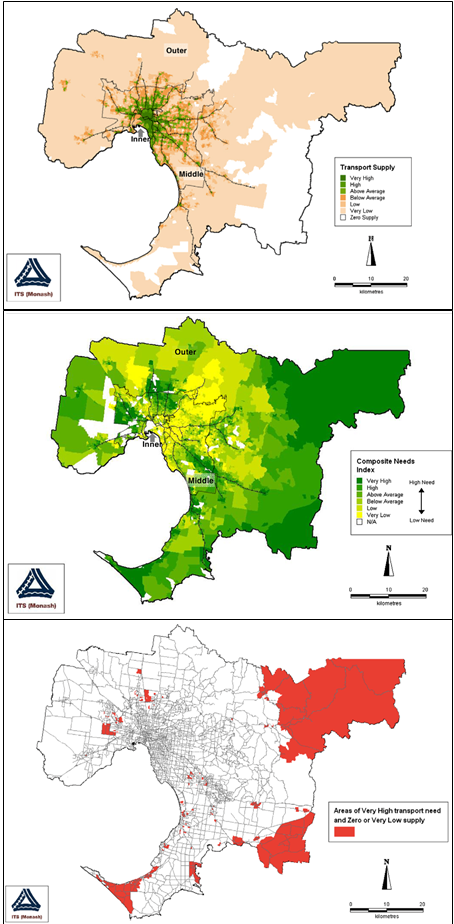
\includegraphics[width=0.9\linewidth]{graphics/Currie2010combined1} \caption{Melbourne 2006: Distribution of supply measure scores (top), needs (middle) and gaps (bottom), Source: Currie (2010)}\label{fig:Currie_map_SI}
\end{figure}

\citet{currie2010identifying} reported SI scores for Census Collection
Districts (CCDs) across Metropolitan Melbourne in 2006, as shown in
Figure \ref{fig:Currie_map_SI}(top). General patterns were identified,
being: more transit supply in the middle and inner suburbs, and along
passenger railway lines; and outer areas tending to have very low SI
scores or no transit supply at all.

\hypertarget{social-need-and-needs-gap}{%
\subsection{Social need and needs-gap}\label{social-need-and-needs-gap}}

As well as measuring transit supply, \citet{currie2010identifying}
assessed the social need for transport across Metropolitan Melbourne
using: the Australian Bureaus of Statistics' Index of Related
Socio-Economic Advantage/Disadvantage (IRSAD) and a transport needs
index derived from eight weighted indicators. The spatial distribution
of this composite social needs index in 2006, reproduced in Figure
\ref{fig:Currie_map_SI}(middle), showed that areas of above average,
high and very high social needs in 2006 were located in: some outer
areas, particularly in the east and south-east; and in some middle areas
in the south-east, north and west.

As the final step in the spatial needs-gap analysis,
\citet{currie2010identifying} identified areas with very high transport
needs, but very low or no transit supply, as reproduced in Figure
\ref{fig:Currie_map_SI}(bottom). These areas were identified as being
those where service gaps might be of particular concern. Most of these
were located in outer parts of Melbourne in the north-east, south-east
and south, although there were also some pockets in the middle suburbs
in the west, north and south east. Overall,
\citet{currie2010identifying} found that ``8.2\% of Melbourne residents
have `very high' needs but `zero', `low' or `very low' public transport
supply.''

Using this methodology in transit planning was suggested as
``substantially more useful than the presentation of anecdotal evidence,
which is the most common means of identifying transport needs in local
transport studies throughout the world'' \citep{currie2010identifying}.
However, it does not appear that this approach has been widely adopted
in practice or by researchers. Our suspicion is that while the SI has a
relatively simple formula and requires only geographic and timetable
data to calculate, a lack of software tools may be partly why it has not
been more widely adopted.

It is also unclear whether the patterns in Melbourne identified in
\citet{currie2010identifying} have changed since the 2006 analysis, or
if Melbourne is representative of other locations. Developing a software
tool to calculate SI tools from GTFS data, and then using it to
comparing current conditions and other locations to the findings of
\citet{currie2010identifying}, therefore, provides motivation for this
research.

\hypertarget{methodology}{%
\section{Methodology}\label{methodology}}

Case research approaches can be particularly useful research questions
are about `how' or `why', but when researchers do not have control of
events (thereby limiting the ability to use experimental
approaches)\citep{Yin2009aa}. In this research the questions relate to
(1) how to use GTFS data to assess gaps between social needs and transit
supply, and (2) how spatial patterns might have changed since those
reported for 2006 in \citet{currie2010identifying}. Addressing the
``duality criterion'' is a key issue when using case research
approaches, this being the need of the research to be seeking
generalisable findings while grounded in the context of only a small
number of cases \citep{Denscombe2007aa, Ketokivi2014aa}. Here the
approach taken has been to develop a package of tools for calculating
the SI from GTFS data using the R programming language \citep{R-base}.
The recommendations of \citet{wickham2023r} informed the package setup
and development approach. Various existing packages and code examples
were relied upon including: the sf package \citep{R-sf} for geospatial
analysis; the tidyverse \citep{tidyverse2019}; gtfstools
\citep{R-gtfstools}; and tidytransit \citep{R-tidytransit}. Using these
methods addresses the duality criterion for the first research question,
as the developed software functions are generic. They are applicable to
other GTFS feeds, and could be used to analyse spatial gaps in transit
supply in other cities, beyond the Melbourne case reported in this
paper.

There are, however, limitations to the generalisability of the findings
of this research with respect to changes since 2006 and the patterns
reported in \citet{currie2010identifying} (research question 2).
\citet{Currie2007Identifying} and \citet{currie2010identifying} reported
results for Melbourne only, and the \citet{Currie2003Hobart} and
\citet{Currie2004Gap} studies of Hobart and Adelaide used earlier
versions of the needs-gap assessment methodology. Hence, it is only
possible to compare Melbourne in 2006 to the Melbourne of now using the
developed code. While this study does seek to findings about changes in
spatial patterns of social need and transit supply that are
generalisable to more than just Melbourne, a lack of 2006 result for
other cities may limit the extent to which these findings might be
considered representative of changes in other places\footnote{Other
  parts of this research programme will examine changes over the last
  10-15 years in cities (where GTFS data is available). The focus of
  this paper, however, is on Melbourne.}.

\hypertarget{code-developement}{%
\subsection{Code developement}\label{code-developement}}

Code was developed and tested on the Mornington Peninsula Tourist
Railway GTFS feed. This was selected primarily for convenience, given
that the authors are familiar with the surrounding geography and that
the feed covers only a small number of trips across just three stations
(thereby facilitating hand verification of outputs).\\
Australian Bureau of Statistics (ABS) data was used to define areas of
interest. This was sourced via the strayr and absmapsdata packages
\citep{r-strayr}.

\hypertarget{melbourne-case-study}{%
\subsection{Melbourne Case Study}\label{melbourne-case-study}}

The methodological literature provides guidance on case study selection
and discussion of various theoretical sampling approaches, including
sampling for critical, particularly revelatory and/or representative
cases
\citep{Eisenhardt1989aa, Yin2009aa, Denscombe2007aa, Eisenhardt2007TBfC}.
\citet{Yin2009aa} notes the selection of a case so as to allow
longitudinal study, and it is this that is the primary reason for the
selection of Melbourne for the research reported in this paper. This
selection allows direct comparison with the 2006 results reported in
\citet{currie2010identifying}, so as to explore the extent to which
spatial patterns of needs-gaps in transit supply have changed over the
last decade and a half. As such, SI scores where calculated using the
same Census Collection Districts (CCDs) used by
\citet{currie2010identifying}, but for the weeks starting the day of the
2016 and 2021 censuses. The Victorian GTFS feed, published by Public
Transport Victoria (PTV), was used, with historical feeds sourced via
\citet{transitfeeds_victoria:2023aa}.

Unfortunately, it is not possible to obtain 2016 or 2021 social
disadvantage data for CCDs, as the Australian Bureau of Statistics (ABS)
no longer releases data using this geographic scheme. Instead,
population and other statistics are now released for Statistical Area 1
(SA1) zones. As such, SI scores have also been calculated for SA1s to
facilitate the use of ABS data. The same Transport Supply
categorizations have been used as in \citet{currie2010identifying}, with
those CCDs/SA1s that have above average SI scores split evenly into
three groups, those that have below average SIs also split evenly into
three groups, and those CCDs/SA1s without SI scores of zero placed in
their own category.

This study adopts a similar approach to measuring social disadvantage as
used in \citet{currie2010identifying}, using: the ABS' Index of Relative
Socio-Economic Advantage/Disadvantage (IRSAD); and a transport needs
index\footnote{The same need indicators and weightings used in
  \citet{currie2010identifying} were adopted, although \$799 or lower
  per week was used as the threshold for low income households rather
  than \$499 to account for inflation (as per the Reserve Bank of
  Australia's online inflation calculator).}. A composite needs
indicator was derived based on the IRSAD and the transport needs index,
again as per the \citet{currie2010identifying} approach. However,
changes to the ABS reporting systems mean that the composite needs
indicator had to be based on weighting both the IRSAD index and the
transport need index by the total population of each SA1 zone, which
were then added, standardised and split into six groups\footnote{This
  contrasts to the method used by \citet{currie2010identifying}, where
  the composite needs index also included relative need components,
  being the IRSAD and the transport needs indexes weighted by the
  population within the various needs groups in each area of interest
  (for a total of four indicators included in the composite needs
  indicator, compared to only two in the 2016 and 2021 results presented
  here.}.

\hypertarget{results}{%
\section{Results}\label{results}}

\hypertarget{the-gtfssupplyindex-package}{%
\subsection{The gtfssupplyindex
Package}\label{the-gtfssupplyindex-package}}

Code developed to calculate SI scores is available as an R package on
github (see \citet{gtfssupplyindex_github}). Included in the package is
a vignette (INCLUDE LINK) that outlines the developed functions and
provides step-by-step calculations for the Mornington Peninsula Railway
as a worked example.

\hypertarget{melbourne}{%
\subsection{Melbourne}\label{melbourne}}

\hypertarget{transport-supply-categories}{%
\subsubsection{Transport Supply
Categories}\label{transport-supply-categories}}

\begin{figure}
\centering
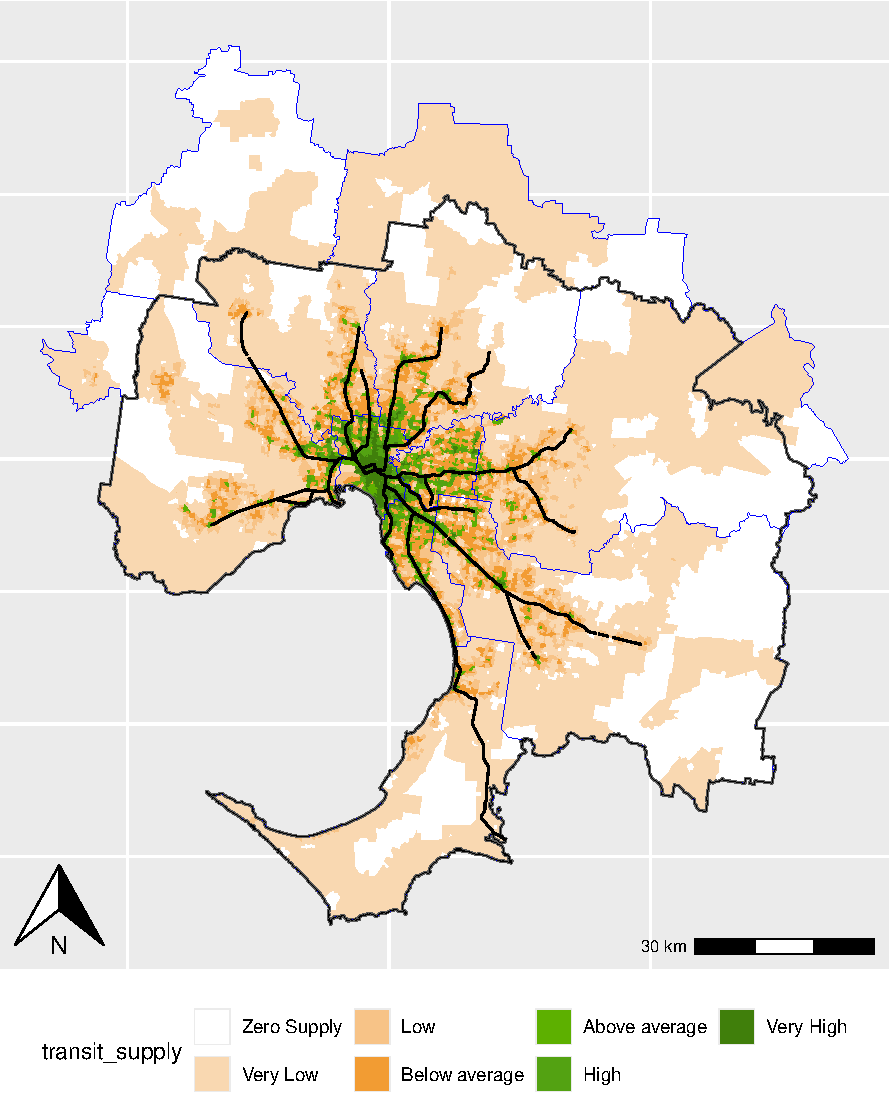
\includegraphics{Leveraging_GTFS_to_assess_transit_supply_Transport_Geography_files/figure-latex/Greater_Melbourne_2021_SA1_plot-1.pdf}
\caption{Greater Melbourne, Transit Supply by SA1 for the week starting
the date of the 2021 census, overlayed with: 2006 Greater Melbourne
boundary (black); 2021 SA4 boundaries (blue); and suburban railway lines
(black)}
\end{figure}

\begin{longtable}[t]{lrrrrr}
\caption{\label{tab:Greater_Melbourne_CCDs_SA1_table}Distribution of 2006, 2016 and 2021 Transport Supply to Melbourne CCDs (2006 boundaries), 2016 Transport Supply to Greater Melbourne (2016 SA1s) and 2021 Transport Supply to Greater Melbourne (2021 SA1s). Sources: 2006 values, Currie (2010); 2016 and 2021 values, authors' analysis}\\
\toprule
\multicolumn{1}{c}{Transport} & \multicolumn{3}{c}{CCDs} & \multicolumn{1}{c}{2016 SA1s} & \multicolumn{1}{c}{2021 SA1s} \\
\cmidrule(l{3pt}r{3pt}){1-1} \cmidrule(l{3pt}r{3pt}){2-4} \cmidrule(l{3pt}r{3pt}){5-5} \cmidrule(l{3pt}r{3pt}){6-6}
Supply & 2006 & 2016 & 2021 & 2016 & 2021\\
\midrule
Zero Supply & 3.2\%   (189) & 1.4\%    (86) & 1.3\%    (81) & 3.2\%    (326) & 4.3\%    (489)\\
Very Low & 22.5\% (1,314) & 23.5\% (1,485) & 23.3\% (1,474) & 23.0\%  (2,362) & 23.4\%  (2,692)\\
Low & 22.4\% (1,310) & 23.5\% (1,484) & 23.3\% (1,473) & 23.0\%  (2,362) & 23.4\%  (2,691)\\
Below average & 22.2\% (1,294) & 23.5\% (1,484) & 23.3\% (1,473) & 23.0\%  (2,362) & 23.4\%  (2,691)\\
Above average & 10.4\%   (608) & 9.4\%   (596) & 9.6\%   (608) & 9.3\%    (959) & 8.5\%    (975)\\
\addlinespace
High & 9.2\%   (535) & 9.4\%   (595) & 9.6\%   (608) & 9.3\%    (959) & 8.5\%    (974)\\
Very High & 10.1\%   (589) & 9.4\%   (595) & 9.6\%   (608) & 9.3\%    (959) & 8.5\%    (975)\\
Total & 100.0\% (5,839) & 100.0\% (6,325) & 100.0\% (6,325) & 100.0\% (10,289) & 100.0\% (11,487)\\
\bottomrule
\end{longtable}

Table \ref{tab:Greater_Melbourne_SA1_2021_table} summarises the
distribution of CCDs and SA1s across different Transport Supply
categories in 2006, 2016 and 2021. Figure
\ref{fig:Greater_Melbourne_2021_SA1_plot} shows the spatial distribution
of Transport Supply in 2021. Maps for 2016 and CCDs are included in the
Appendix.

Differences in the shares of CCDs in each category in 2006, 2016 and
2021 are statistically significant (\(\chi^2(12, N = 18489) = 87.45\),
\(p < .001\)). Only 81 CCDs (1.3\%) have Zero Supply in 2021, compared
to the 189 (3.2\%) reported by \citet{currie2010identifying} for 2006.
Differences are also statistically significant when comparing 2006 and
2016 (\(\chi^2(6, N = 12164) = 56.87\), \(p < .001\) or 2006 and 2021
\(\chi^2(6, N = 12164) = 59.15\), \(p < .001\), but not between 2016 and
2021 (\(\chi^2(6, N = 12650) = 0.67\), \(p = .995\)).

These values, however, are for CCDs within the 2006 extents of
Melbourne. The ABS' statistical boundary of ``Greater Melbourne'' now
includes areas up to around 30 kilometers further to the north, as shown
in the 2021 map in Figure \ref{fig:Greater_Melbourne_2021_SA1_plot}.
This shows that the new parts of Melbourne, beyond the 2006 statistical
boundary, mostly have Very Low or Zero Transport Supply levels. Again,
the differences between 2006 (CCDs), 2016 and 2021 (SA1s) are
statistically significant (\(\chi^2(12, N = 27615) = 58.86\),
\(p < .001\)) as are the difference when comparing each pair (2006 vs
2016, \(\chi^2(6, N = 16128) = 8.83\), \(p = .183\); 2006 vs 2021
\(\chi^2(6, N = 17326) = 44.83\), \(p < .001\); and 2016 vs 2021
\(\chi^2(6, N = 21776) = 31.56\), \(p < .001\)). There are a greater
proportion of SA1s with Zero Supply in 2021 (4.3\%) than there were CCDs
in 2006 (3.25\%). The share of SA1s with supply below the average SI
score (i.e.~Zero, Very Low, Low or Below Average) is also larger in 2021
(74.5\%) compared to the share of CCDs in 2006 (70.3\%).

\begin{longtable}[]{@{}
  >{\raggedright\arraybackslash}p{(\columnwidth - 6\tabcolsep) * \real{0.1972}}
  >{\raggedleft\arraybackslash}p{(\columnwidth - 6\tabcolsep) * \real{0.2676}}
  >{\raggedleft\arraybackslash}p{(\columnwidth - 6\tabcolsep) * \real{0.2676}}
  >{\raggedleft\arraybackslash}p{(\columnwidth - 6\tabcolsep) * \real{0.2676}}@{}}
\caption{Distribution of 2006, 2016 and 2021 Transport Supply to
population in Melbourne. Sources: 2006 values, Currie (2010); 2016 and
2021 values, authors' analysis}\tabularnewline
\toprule\noalign{}
\begin{minipage}[b]{\linewidth}\raggedright
Supply
\end{minipage} & \begin{minipage}[b]{\linewidth}\raggedleft
2006
\end{minipage} & \begin{minipage}[b]{\linewidth}\raggedleft
2016
\end{minipage} & \begin{minipage}[b]{\linewidth}\raggedleft
2021
\end{minipage} \\
\midrule\noalign{}
\endfirsthead
\toprule\noalign{}
\begin{minipage}[b]{\linewidth}\raggedright
Supply
\end{minipage} & \begin{minipage}[b]{\linewidth}\raggedleft
2006
\end{minipage} & \begin{minipage}[b]{\linewidth}\raggedleft
2016
\end{minipage} & \begin{minipage}[b]{\linewidth}\raggedleft
2021
\end{minipage} \\
\midrule\noalign{}
\endhead
\bottomrule\noalign{}
\endlastfoot
Zero Supply & 2.5\% (85,423) & 2.9\% (131,619) & 3.8\% (186,829) \\
Very Low & 23.6\% (793,046) & 22.5\% (1,008,498) & 23.0\% (1,132,967) \\
Low & 25.7\% (865,330) & 22.7\% (1,016,848) & 23.7\% (1,163,358) \\
Below average & 23.0\% (774,521) & 22.3\% (1,000,290) & 23.6\%
(1,159,783) \\
Above average & 9.6\% (324,546) & 9.3\% (418,614) & 8.7\% (426,892) \\
High & 7.7\% (260,411) & 9.6\% (428,880) & 8.7\% (425,779) \\
Very High & 7.8\% (263,832) & 10.7\% (480,469) & 8.6\% (422,025) \\
Total & 100.0\% (3,367,109) & 100.0\% (4,485,218) & 100.0\%
(4,917,633) \\
\end{longtable}

Table \ref{tab:Greater_Melbourne_CCDs_SA1_population} compares the share
of resident population in each transport supply category. Differences
are statistically significant across 2006 and 2021
(\(\chi^2(6, N = 8284742) = 19038.97\), \(p < .001\)). The number of
people with zero supply rose from 85,423 (2.5\%) in 2006 to 186,829
(3.8\%) in 2021. This represents a 118.7\% increase, compared to the
population increase of 46.0\% across all of Greater Melbourne. The
number of people with zero or very low supply rose from 878,469 (26.1\%)
in 2006 to 1,319,796 (26.8\%) in 2021. This represents a 50.2\% increase
(4.2\% higher than the population change). The number of people with a
supply that was below the average (Zero, Very Low, Low or Below Average)
rose from 2,518,320 (74.8\%) in 2006 to 3,642,937 (74.1\%) in 2021. This
represents a 44.7\% increase (1.4\% lower than the population change).

Differences were also statistically significant between 2016 and 2021
(\(\chi^2(6, N = 9402851) = 22467.17\), \(p < .001\)). The number of
people with zero supply rose from 131,619 (2.9\%) in 2016 (+55,210,
+41.9\%, compared to the population increase of 9.6\% across all of
Greater Melbourne. The number of people with zero or very low supply
rose from 1,140,117 (25.4\%) (+179,679, +15.8\%), while the number with
a supply that was below the average (Zero, Very Low, Low or Below
Average) rose from 3,157,255 (70.4\%) in 2016 (+ 485,682, 15.4\%).

\begingroup\fontsize{8}{10}\selectfont

\begin{longtable}[t]{>{\raggedright\arraybackslash}p{1.75cm}>{\raggedleft\arraybackslash}p{1cm}>{\raggedleft\arraybackslash}p{1cm}>{\raggedleft\arraybackslash}p{1cm}>{\raggedleft\arraybackslash}p{1cm}>{\raggedleft\arraybackslash}p{1cm}>{\raggedleft\arraybackslash}p{1cm}>{\raggedleft\arraybackslash}p{1cm}>{\raggedright\arraybackslash}p{1cm}>{\raggedleft\arraybackslash}p{1cm}>{\raggedleft\arraybackslash}p{1.25cm}}
\caption{\label{tab:Greater_Melbourne_population_2016_by_SA4}Greater Melbourne 2016: Share of population in each Transport Supply category for each SA4 region}\\
\toprule
transit\_supply & Inner & Inner East & Inner South & North East & North West & Outer East & South East & West & Mornington Peninsula & Total\\
\midrule
Zero Supply & 0.0\%       (0) & 0.0\%     (480) & 0.0\%   (1,604) & 0.4\%  (16,988) & 0.4\%  (17,655) & 0.3\%  (12,955) & 1.0\%  (44,757) & 0.3\%  (12,056) & 0.6\%  (25,124) & 2.9\%   (131,619)\\
Very Low & 0.1\%   (3,427) & 0.4\%  (18,454) & 0.6\%  (24,944) & 2.5\% (112,269) & 2.1\%  (94,853) & 4.3\% (190,890) & 4.8\% (215,217) & 4.2\% (186,665) & 3.6\% (161,779) & 22.5\% (1,008,498)\\
Low & 0.4\%  (18,018) & 0.9\%  (39,235) & 1.4\%  (60,833) & 2.7\% (119,608) & 2.4\% (107,693) & 3.0\% (135,247) & 5.0\% (224,097) & 5.4\% (242,438) & 1.6\%  (69,679) & 22.7\% (1,016,848)\\
Below average & 1.0\%  (42,950) & 2.3\% (105,168) & 2.9\% (128,014) & 2.9\% (132,008) & 2.2\%  (97,739) & 2.7\% (119,691) & 4.0\% (177,817) & 3.8\% (170,015) & 0.6\%  (26,888) & 22.3\% (1,000,290)\\
Above average & 1.0\%  (44,547) & 1.8\%  (80,002) & 1.8\%  (81,038) & 1.0\%  (46,965) & 0.6\%  (28,905) & 0.6\%  (25,188) & 1.2\%  (53,228) & 1.2\%  (54,895) & 0.1\%   (3,846) & 9.3\%   (418,614)\\
\addlinespace
High & 2.9\% (129,533) & 1.7\%  (74,966) & 1.7\%  (74,617) & 1.0\%  (46,291) & 0.3\%  (14,464) & 0.3\%  (15,371) & 0.7\%  (33,365) & 0.9\%  (38,499) & 0.0\%   (1,774) & 9.6\%   (428,880)\\
Very High & 7.9\% (353,232) & 0.9\%  (41,416) & 0.7\%  (32,561) & 0.5\%  (21,197) & 0.0\%   (2,033) & 0.0\%     (314) & 0.2\%   (6,893) & 0.5\%  (22,823) & 0.0\%       (0) & 10.7\%   (480,469)\\
Total & 13.2\% (591,707) & 8.0\% (359,721) & 9.0\% (403,611) & 11.0\% (495,326) & 8.1\% (363,342) & 11.1\% (499,656) & 16.8\% (755,374) & 16.2\% (727,391) & 6.4\% (289,090) & 100.0\% (4,485,218)\\
\bottomrule
\end{longtable}
\endgroup{}

\begingroup\fontsize{8}{10}\selectfont

\begin{longtable}[t]{>{\raggedright\arraybackslash}p{1.75cm}>{\raggedleft\arraybackslash}p{1cm}>{\raggedleft\arraybackslash}p{1cm}>{\raggedleft\arraybackslash}p{1cm}>{\raggedleft\arraybackslash}p{1cm}>{\raggedleft\arraybackslash}p{1cm}>{\raggedleft\arraybackslash}p{1cm}>{\raggedleft\arraybackslash}p{1cm}>{\raggedright\arraybackslash}p{1cm}>{\raggedleft\arraybackslash}p{1cm}>{\raggedleft\arraybackslash}p{1.25cm}}
\caption{\label{tab:Greater_Melbourne_population_2021_by_SA4}Greater Melbourne 2021: Share of population in each Transport Supply category for each SA4 region}\\
\toprule
transit\_supply & Inner & Inner East & Inner South & North East & North West & Outer East & South East & West & Mornington Peninsula & Total\\
\midrule
Zero Supply & 0.0\%       (0) & 0.3\%     (478) & 0.9\%   (1,655) & 14.2\%  (26,563) & 11.9\%  (22,186) & 7.6\%  (14,125) & 28.9\%  (53,966) & 23.5\%  (43,898) & 12.8\%  (23,958) & 100.0\%   (186,829)\\
Very Low & 0.4\%   (4,169) & 1.8\%  (20,688) & 2.0\%  (22,483) & 11.5\% (130,715) & 9.8\% (110,814) & 17.7\% (200,810) & 22.1\% (250,684) & 19.5\% (221,337) & 15.1\% (171,267) & 100.0\% (1,132,967)\\
Low & 1.7\%  (20,329) & 3.9\%  (45,160) & 5.5\%  (63,802) & 11.3\% (132,001) & 10.6\% (123,314) & 13.4\% (155,603) & 22.9\% (265,995) & 24.9\% (289,518) & 5.8\%  (67,636) & 100.0\% (1,163,358)\\
Below average & 4.7\%  (54,918) & 11.5\% (133,305) & 12.8\% (148,585) & 13.0\% (151,240) & 11.2\% (129,918) & 9.9\% (114,658) & 17.6\% (204,093) & 15.9\% (184,466) & 3.3\%  (38,600) & 100.0\% (1,159,783)\\
Above average & 13.2\%  (56,422) & 16.2\%  (69,199) & 21.8\%  (92,875) & 10.4\%  (44,470) & 6.4\%  (27,140) & 5.2\%  (22,262) & 12.5\%  (53,328) & 13.0\%  (55,438) & 1.3\%   (5,758) & 100.0\%   (426,892)\\
\addlinespace
High & 35.6\% (151,439) & 17.3\%  (73,687) & 16.3\%  (69,281) & 10.3\%  (43,985) & 2.3\%   (9,710) & 2.6\%  (10,905) & 5.8\%  (24,707) & 9.7\%  (41,100) & 0.2\%     (965) & 100.0\%   (425,779)\\
Very High & 78.1\% (329,654) & 7.3\%  (30,949) & 5.7\%  (23,906) & 2.8\%  (11,752) & 0.3\%   (1,285) & 0.0\%       (0) & 1.7\%   (7,308) & 4.1\%  (17,171) & 0.0\%       (0) & 100.0\%   (422,025)\\
Total & 12.5\% (616,931) & 7.6\% (373,466) & 8.6\% (422,587) & 11.0\% (540,726) & 8.6\% (424,367) & 10.5\% (518,363) & 17.5\% (860,081) & 17.3\% (852,928) & 6.3\% (308,184) & 100.0\% (4,917,633)\\
\bottomrule
\end{longtable}
\endgroup{}

Table \ref{tab:Greater_Melbourne_population_2016_by_SA4} and Table
\ref{tab:Greater_Melbourne_population_2021_by_SA4} show the distribution
of Transport Supply categories to the population in each SA4 zone in
2016 and 2021 respectively. Variations across SA4 zones are
statistically significant in both 2016
(\(\chi^2(48, N = 4485218) = 2847273.25\), \(p < .001\)) and 2021
(\(\chi^2(48, N = 4917633) = 3126013.64\), \(p < .001\)). In general,
outer areas of Greater Melbourne\footnote{The North East, North West,
  Outer East, South East, West and Mornington Peninsula SA4 zones}
appear to have larger shares of residents living in areas with Transport
Supply that is lower than the average. In 2016 2,714,128 residents
(60.5\%) lived outside of the inner three SA4 areas and had lower than
average transport supply. By 2021 this had increased to 3,127,365
residents (63.6\%).

\hypertarget{supply-index-scores}{%
\subsubsection{Supply Index scores}\label{supply-index-scores}}

\citet{currie2010identifying} reported an average SI score for CCDs in
2006 was 2,886.9 across Melbourne. Within the same (2006) boundary the
average SI value in 2021 (using CCDs) was 3,390 indicating that the
overall transit service supply score has increased by approximately
31\%. SI scores average 12,275.7, 3,409.1 and 998.96 in 2021 for the
CCDs in the inner, middle and outer suburbs respectively\footnote{The
  same grouping of LGAs to inner, middle and outer suburb groups as used
  in \citet{currie2010identifying} was used for this analysis, although
  here the City of Stonnington was allocated entirely to the middle
  grouping, whereas \citet{currie2010identifying} allocated part of this
  LGA to the inner group.}, compared to 10,922.7, 2,694.9 and 764.3,
respectively, reported for 2006 in \citet{currie2010identifying}.

Comparing SA1s across all of Greater Melbourne, average SI scores
increased from 2,843.8 in 2016 to 2,901.4 in 2021 (+2.0\%). There is a
significant and strong correlation between the 2016 and 2021 SI scores
(\(r_s =.98\), \(p < .001\)).

\begingroup\fontsize{8}{10}\selectfont

\begin{longtable}[t]{>{\raggedright\arraybackslash}p{1.75cm}>{\raggedleft\arraybackslash}p{1cm}>{\raggedleft\arraybackslash}p{1cm}>{\raggedleft\arraybackslash}p{1cm}>{\raggedleft\arraybackslash}p{1cm}>{\raggedleft\arraybackslash}p{1cm}>{\raggedleft\arraybackslash}p{1cm}>{\raggedleft\arraybackslash}p{1cm}>{\raggedright\arraybackslash}p{1cm}>{\raggedleft\arraybackslash}p{1cm}>{\raggedleft\arraybackslash}p{1.25cm}}
\caption{\label{tab:Greater_Melbourne_2016_2021_ratio_map}Greater Melbourne: Share of 2021 population living in SA1s by change in transit service (2016 vs 2021) by SA4 region}\\
\toprule
Change & Inner & Inner East & Inner South & North East & North West & Outer East & South East & West & M'ton P'sula & Total\\
\midrule
Never served & 0.0\%       (0) & 0.0\%     (478) & 0.0\%   (1,655) & 0.5\%  (24,786) & 0.4\%  (21,762) & 0.3\%  (12,855) & 1.1\%  (52,606) & 0.9\%  (42,883) & 0.5\%  (23,958) & 3.7\%   (180,983)\\
New service & 0.0\%       (0) & 0.0\%       (0) & 0.0\%       (0) & 0.2\%   (9,911) & 0.7\%  (36,817) & 0.0\%     (238) & 1.1\%  (53,254) & 0.8\%  (40,483) & 0.1\%   (3,038) & 2.9\%   (143,741)\\
Increased 30\% or more & 0.0\%   (1,843) & 0.0\%     (279) & 0.8\%  (37,932) & 0.9\%  (46,448) & 1.7\%  (83,007) & 0.1\%   (4,209) & 2.6\% (127,248) & 2.7\% (131,194) & 1.3\%  (65,724) & 10.1\%   (497,884)\\
Increased 10 to 30\% & 0.9\%  (45,197) & 0.1\%   (3,190) & 0.8\%  (41,577) & 0.8\%  (40,989) & 1.1\%  (56,013) & 0.5\%  (22,609) & 1.6\%  (77,391) & 2.1\% (101,767) & 0.4\%  (21,060) & 8.3\%   (409,793)\\
Increased 5 to 10\% & 1.5\%  (72,360) & 0.3\%  (13,018) & 1.1\%  (52,033) & 0.8\%  (37,258) & 0.6\%  (31,400) & 0.5\%  (26,666) & 1.1\%  (53,370) & 2.1\% (101,769) & 0.2\%  (10,149) & 8.1\%   (398,023)\\
\addlinespace
Increased 3 to 5\% & 1.6\%  (79,047) & 0.5\%  (25,074) & 0.6\%  (30,595) & 1.2\%  (60,661) & 1.1\%  (55,445) & 0.5\%  (23,819) & 0.9\%  (45,773) & 1.8\%  (88,601) & 0.3\%  (14,666) & 8.6\%   (423,681)\\
Increased 1 to 3\% & 2.3\% (115,203) & 1.4\%  (67,357) & 1.2\%  (60,889) & 1.9\%  (92,896) & 0.9\%  (42,761) & 0.8\%  (39,263) & 1.5\%  (75,676) & 2.4\% (117,967) & 0.7\%  (32,811) & 13.1\%   (644,823)\\
Within 1\% & 2.6\% (128,666) & 3.8\% (187,974) & 2.0\%  (97,037) & 2.5\% (124,942) & 1.2\%  (57,899) & 5.6\% (274,423) & 5.4\% (266,787) & 3.0\% (146,702) & 2.2\% (109,151) & 28.3\% (1,393,581)\\
Reduced 1 to 3\% & 1.0\%  (49,729) & 0.8\%  (39,675) & 0.6\%  (27,179) & 0.7\%  (34,180) & 0.3\%  (13,986) & 0.8\%  (38,826) & 0.7\%  (34,125) & 0.4\%  (19,517) & 0.4\%  (18,446) & 5.6\%   (275,663)\\
Reduced 3 to 10\% & 1.8\%  (89,662) & 0.5\%  (25,930) & 0.9\%  (42,701) & 0.9\%  (44,261) & 0.2\%  (11,175) & 0.9\%  (43,143) & 0.5\%  (24,903) & 0.7\%  (33,329) & 0.2\%   (7,953) & 6.6\%   (323,057)\\
\addlinespace
Reduced by more than 10\% & 0.7\%  (35,224) & 0.2\%  (10,491) & 0.6\%  (30,989) & 0.5\%  (22,617) & 0.3\%  (13,678) & 0.6\%  (31,042) & 1.0\%  (47,588) & 0.6\%  (27,701) & 0.0\%   (1,228) & 4.5\%   (220,558)\\
Service withdrawn & 0.0\%       (0) & 0.0\%       (0) & 0.0\%       (0) & 0.0\%   (1,777) & 0.0\%     (424) & 0.0\%   (1,270) & 0.0\%   (1,360) & 0.0\%   (1,015) & 0.0\%       (0) & 0.1\%     (5,846)\\
Total & 12.5\% (616,931) & 7.6\% (373,466) & 8.6\% (422,587) & 11.0\% (540,726) & 8.6\% (424,367) & 10.5\% (518,363) & 17.5\% (860,081) & 17.3\% (852,928) & 6.3\% (308,184) & 100.0\% (4,917,633)\\
\bottomrule
\end{longtable}
\endgroup{}

\begin{figure}
\centering
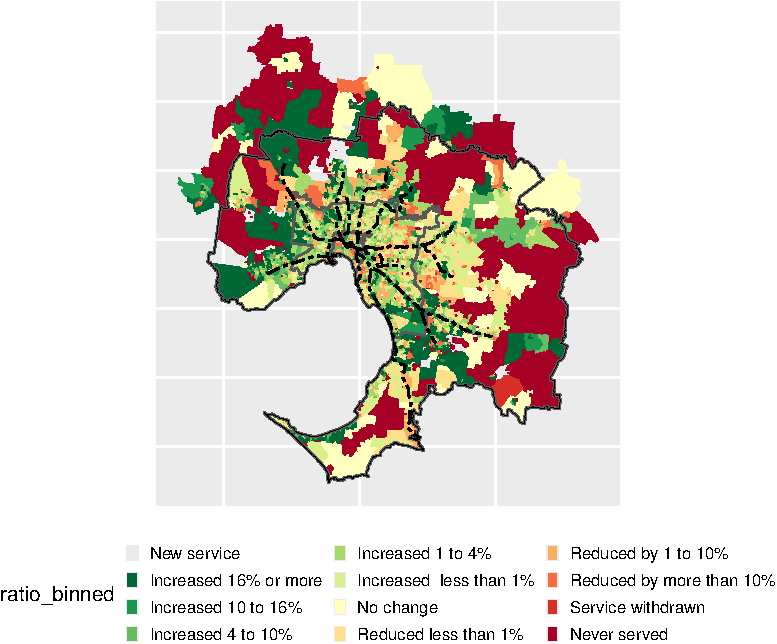
\includegraphics{Leveraging_GTFS_to_assess_transit_supply_Transport_Geography_files/figure-latex/Greater_Melbourne_2016_2021_ratio_map-1.pdf}
\caption{Greater Melbourne: changes in SI between 2016 and 2021, by SA1,
overlayed with 2006 Melbourne boundary (black), SA4 boundaries (blue)
and suburban railway lines (black)}
\end{figure}

Table \ref{tab:Greater_Melbourne_2016_2021_ratio_population_table} shows
changes in SI score between 2016 and 2021 (column 1) by SA1s for the
2021 population, summarised for each SA4 zone (columns 2 to 10) and
Greater Melbourne as a whole (column 11). These are mapped in Figure
\ref{fig:Greater_Melbourne_2016_2021_ratio_map}. There is a
statistically significant difference in the distribution of service
level changes across the populations in each SA4 area
(\(\chi^2(88, N = 4917633) = 1220826.77\), \(p < .001\)). More than half
of the population in the North-West, West, North East, South East,
Mornginton Peninsula and Inner areas of Melbourne had increased service
levels in 2021 compared to 2016, while service levels remained within
one percent for 52.9\% of the population in the Outer East and 50.3\%.
More of the population had less service in 2021 than 2016 in the Inner
(28.3\%), Inner South (23.9\%) and Outer East (22.0\%). In terms of
overall population, however, the largest shares to have more service in
2021 were in the west (581,781 residents in 2021), South East (432,712)
and the Inner (313,650) SA4 areas. The largest shares of residents with
a lower service level in 2021 were amongst the Inner (174,615), Outer
East (114,281) and South East (107,976) SA4 areas.

\hypertarget{social-needs}{%
\subsubsection{Social needs}\label{social-needs}}

\begin{figure}
\centering
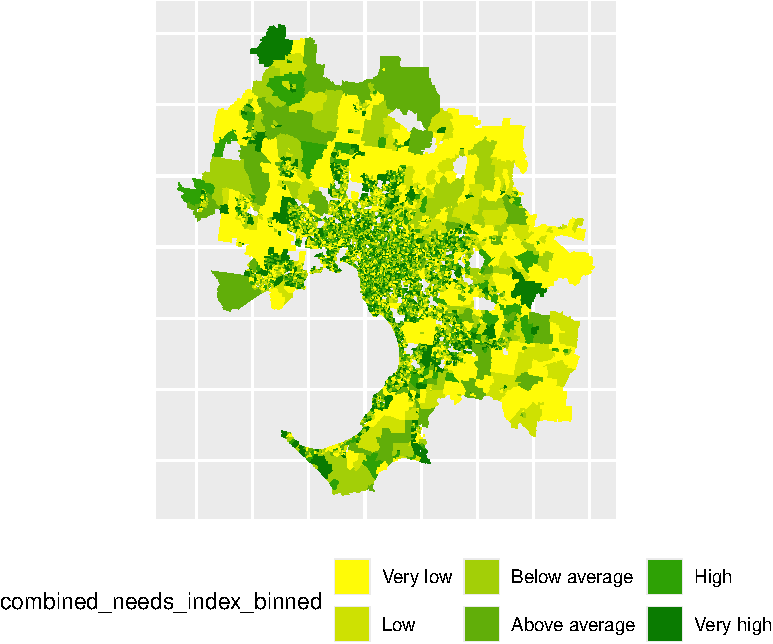
\includegraphics{Leveraging_GTFS_to_assess_transit_supply_Transport_Geography_files/figure-latex/Greater_Melbourne_2021_social_needs-1.pdf}
\caption{Distribution of categories of composite social need index
scores, overlayed with: 2006 Greater Melbourne boundary (black); SA4
boundaries (blue); and suburban railway lines (dashed).}
\end{figure}

Figure \ref{fig:Greater_Melbourne_2021_social_needs} shows the
distribution of categories of social need index scores across Greater
Melbourne for 2021\^{}{[}A map for 2016 is included in the Appendix as
Figure \ref{Greater_Melbourne_2016_social_needs_appendix}. This is
analagous to the 2006 map shown in Figure
\ref{fig:Currie_map_SI}(middle), although as discussed in the
methodology section above, it was not possible to exactly replicate the
\citet{currie2010identifying} approach due to changes in the way census
results are reported. In general, the spatial grouping of different
levels of social need appears less consistent in 2021 than in 2006.
However, this may be an artifact of the shift to SA1s from
CCDs\footnote{CCDs were originally devised to group the approximately
  200 dwellings allocated to each individual census collector, whereas
  SA1s were introduced in be consistent in population (200 to 800
  people, averaging 400) and character\citep{ABS_SA1s_CCDs}}.

\hypertarget{needs-gap}{%
\subsubsection{Needs-gap}\label{needs-gap}}

\begin{figure}
\centering
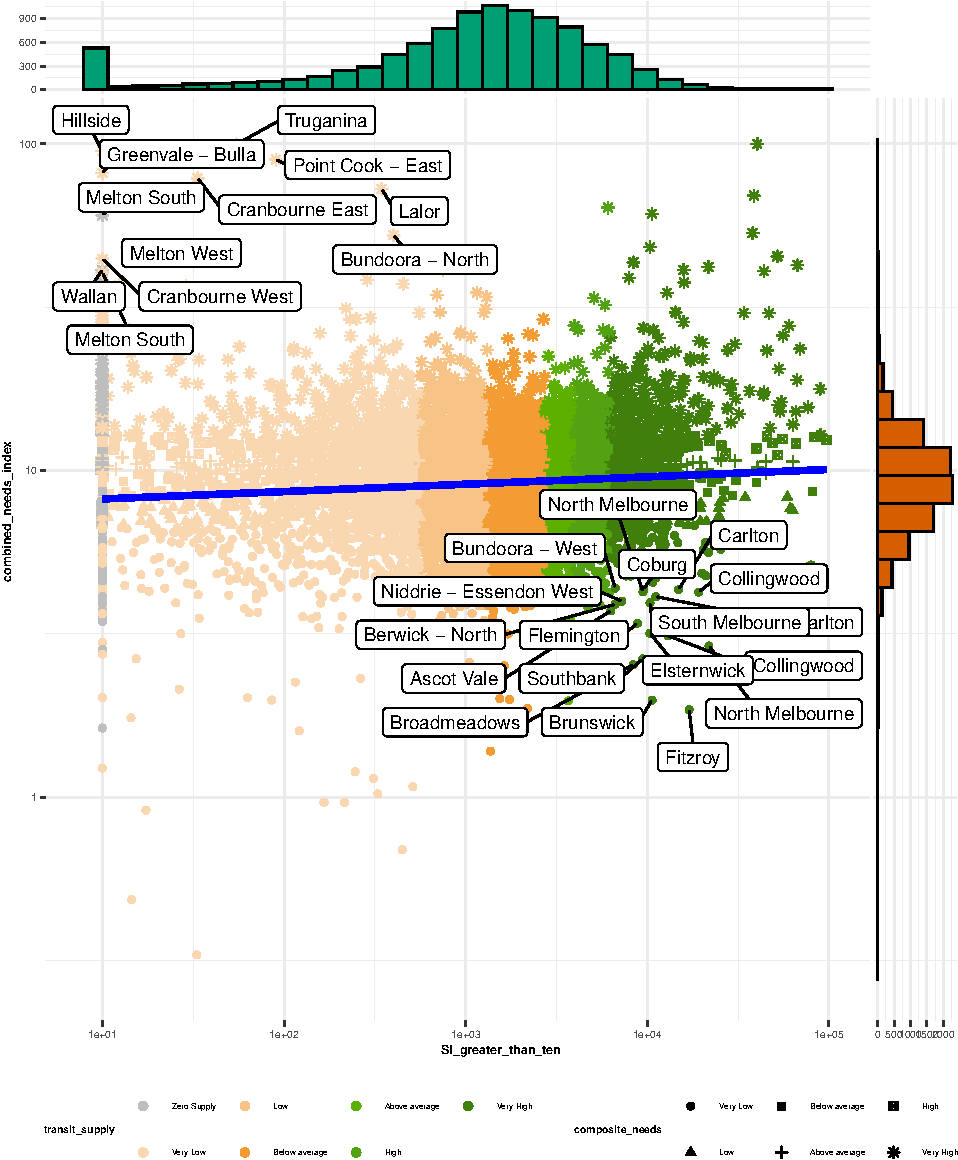
\includegraphics{Leveraging_GTFS_to_assess_transit_supply_Transport_Geography_files/figure-latex/Greater_Melbourne_2016_needs_gap_scatterplot_figure-1.pdf}
\caption{Greater Melbourne 2016, SI and Combined Needs Index scores,
with SI scores \textless{} 10 rounded up to equal 10.}
\end{figure}

\begin{figure}
\centering
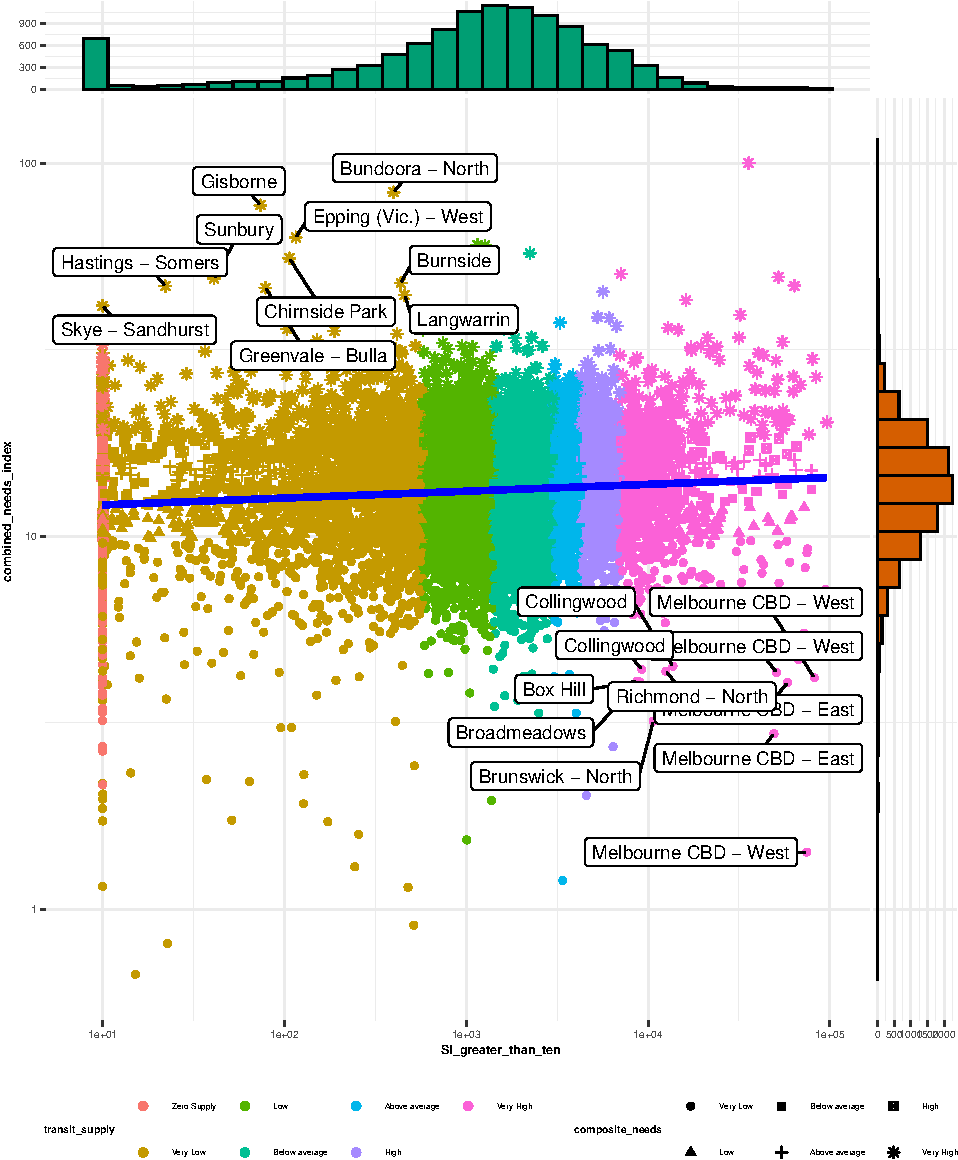
\includegraphics{Leveraging_GTFS_to_assess_transit_supply_Transport_Geography_files/figure-latex/Greater_Melbourne_2021_needs_gap_scatterplot_figure-1.pdf}
\caption{Greater Melbourne 2016, SI and Combined Needs Index scores,
with SI scores \textless{} 10 rounded up to equal 10.}
\end{figure}

Figures \ref{fig:Greater_Melbourne_2016_needs_gap_scatterplot_figure}
and \ref{fig:Greater_Melbourne_2016_needs_gap_scatterplot_figure} show
social needs and SI scores\footnote{To improve the clarity of the
  figure, SI scores less than 10 have been adjusted to equal 10.}. There
is a significant, but only weakly positive correlation between the SI
and Combined Needs Index scores for both 2016 (\(r_s =.07\),
\(p < .001\)) and 2021 (\(r_s =.07\), \(p < .001\)).

Table \ref{tab:Greater_Melbourne_2016_needs_gap_zones_tables} shows
Differences in the share of groupings across categories is statistically
significant (\(\chi^2(30, N = 9964) = 264.26\), \(p < .001\)), with more
of the SA1s with higher needs tending to have transport supplies that
are higher than the average. 365 SA1s have Zero or Very Low transport
supply, but very high social needs. This represents 3.7\% of the 9,964
SA1s within Greater Melbourne, and is a lower proportion than that
reported for 2006 (279 of 5,720 CCDs (4.9\%)) in
\citet{currie2010identifying}.

Table \ref{tabGreater_Melbourne_2021_needs_gap_zones_tables} Differences
in the share of groupings across categories is statistically significant
(\(\chi^2(30, N = 11138) = 133.51\), \(p < .001\)), with more of the
SA1s with higher needs tending to have transport supplies that are
higher than the average. 469 SA1s have Zero or Very Low transport
supply, but very high social needs. This represents 4.2\% of the 11,138
SA1s within Greater Melbourne, and is a lower proportion than that
reported for 2006 (279 of 5,720 CCDs (4.9\%)) in
\citet{currie2010identifying}.

\begingroup\fontsize{7}{9}\selectfont

\begin{longtable}[t]{lrrrrrrr}
\caption{\label{tab:Greater_Melbourne_2016_needs_gap_zones}Greater Melbourne 2016, SA1s within each SI and Combined Needs Index grouping}\\
\toprule
transit\_supply & Very Low & Low & Below average & Above average & High & Very High & Total\\
\midrule
Zero Supply & 4.8\%    (91) & 3.5\%    (66) & 2.5\%    (47) & 2.4\%    (34) & 2.0\%    (28) & 3.2\%    (46) & 3.1\%   (312)\\
Very Low & 26.1\%   (497) & 23.2\%   (442) & 20.9\%   (397) & 20.4\%   (290) & 19.8\%   (281) & 22.5\%   (319) & 22.3\% (2,226)\\
Low & 24.1\%   (458) & 24.5\%   (467) & 24.4\%   (464) & 22.3\%   (317) & 21.7\%   (308) & 19.7\%   (279) & 23.0\% (2,293)\\
Below average & 24.9\%   (473) & 24.5\%   (467) & 24.1\%   (459) & 23.8\%   (338) & 23.2\%   (329) & 17.6\%   (249) & 23.2\% (2,315)\\
Above average & 7.4\%   (140) & 9.2\%   (175) & 10.2\%   (194) & 10.5\%   (149) & 10.6\%   (150) & 9.2\%   (131) & 9.4\%   (939)\\
\addlinespace
High & 6.5\%   (123) & 7.5\%   (142) & 10.7\%   (203) & 10.2\%   (145) & 12.0\%   (170) & 10.9\%   (155) & 9.4\%   (938)\\
Very High & 6.4\%   (121) & 7.6\%   (144) & 7.3\%   (139) & 10.3\%   (146) & 10.7\%   (152) & 16.9\%   (239) & 9.4\%   (941)\\
Total & 100.0\% (1,903) & 100.0\% (1,903) & 100.0\% (1,903) & 100.0\% (1,419) & 100.0\% (1,418) & 100.0\% (1,418) & 100.0\% (9,964)\\
\bottomrule
\end{longtable}
\endgroup{}

\begingroup\fontsize{7}{9}\selectfont

\begin{longtable}[t]{lrrrrrrr}
\caption{\label{tab:Greater_Melbourne_2021_needs_gap_zones}Greater Melbourne 2021, SA1s within each SI and Combined Needs Index grouping}\\
\toprule
transit\_supply & Very Low & Low & Below average & Above average & High & Very High & Total\\
\midrule
Zero Supply & 6.4\%   (130) & 4.7\%    (95) & 3.9\%    (79) & 2.9\%    (49) & 3.0\%    (51) & 3.6\%    (61) & 4.2\%    (465)\\
Very Low & 25.6\%   (521) & 22.2\%   (452) & 21.8\%   (444) & 21.0\%   (352) & 22.0\%   (369) & 24.3\%   (408) & 22.9\%  (2,546)\\
Low & 23.5\%   (479) & 25.3\%   (514) & 24.6\%   (500) & 24.0\%   (403) & 22.4\%   (376) & 20.6\%   (346) & 23.5\%  (2,618)\\
Below average & 23.7\%   (483) & 23.7\%   (482) & 24.0\%   (488) & 25.6\%   (430) & 24.6\%   (412) & 20.8\%   (349) & 23.7\%  (2,644)\\
Above average & 6.9\%   (140) & 8.1\%   (165) & 9.2\%   (188) & 9.4\%   (157) & 9.1\%   (152) & 9.2\%   (154) & 8.6\%    (956)\\
\addlinespace
High & 5.9\%   (120) & 8.0\%   (162) & 9.5\%   (193) & 9.2\%   (154) & 9.7\%   (162) & 9.8\%   (165) & 8.6\%    (956)\\
Very High & 8.0\%   (163) & 8.1\%   (165) & 7.0\%   (143) & 7.9\%   (133) & 9.2\%   (155) & 11.6\%   (194) & 8.6\%    (953)\\
Total & 100.0\% (2,036) & 100.0\% (2,035) & 100.0\% (2,035) & 100.0\% (1,678) & 100.0\% (1,677) & 100.0\% (1,677) & 100.0\% (11,138)\\
\bottomrule
\end{longtable}
\endgroup{}

Table \ref{tab:Greater_Melbourne_2016_needs_gap_population} compares the
populations within each SI and Combined Needs Index grouping for 2016.
There is a statistically significant relationship
(\(\chi^2(30, N = 4471171) = 158778.27\), \(p < .001\)), with more of
the population that has higher needs tending to be living in SA1s that
have transport supplies that ave higher than the average. 301,743 people
live within SA1s that have Zero or Very Low transport supply, but Very
High social needs. This represents 6.7\% of the 4,471,171 people within
Greater Melbourne, and is higher proportion than that reported for 2006
(139,004 of 3.3 million people (4.2\%)).

Table \ref{tab:Greater_Melbourne_2021_needs_gap_population} compares the
populations within each SI and Combined Needs Index grouping for 2021.
There is a statistically significant relationship
(\(\chi^2(30, N = 4904313) = 55715.62\), \(p < .001\)), with more of the
population that has higher needs tending to be living in SA1s that have
transport supplies that ave higher than the average. 333,887 people live
within SA1s that have Zero or Very Low transport supply, but Very High
social needs. This represents 6.8\% of the 4,904,313 people within
Greater Melbourne, and is higher proportion than that reported for 2006
(139,004 of 3.3 million people (4.2\%)).

\begingroup\fontsize{6}{8}\selectfont

\begin{longtable}[t]{lrrrlrrr}
\caption{\label{tab:Greater_Melbourne_2016_needs_gap_population}Greater Melbourne 2016, Population in each SI and Combined Needs Index grouping}\\
\toprule
\multicolumn{1}{c}{ } & \multicolumn{6}{c}{Combined Needs Index Category} & \multicolumn{1}{c}{ } \\
\cmidrule(l{3pt}r{3pt}){2-7}
Supply & Very High & High & Above Average & Below Average & Low & Very Low & Total\\
\midrule
Zero Supply & 0.9\%    (38,050) & 0.3\%  (14,790) & 0.3\%  (15,402) & 0.4\%  (18,784) & 0.5\%  (22,544) & 0.5\%  (22,012) & 2.9\%   (131,582)\\
Very Low & 5.9\%   (263,693) & 3.4\% (153,169) & 3.1\% (138,710) & 3.7\% (165,350) & 3.5\% (156,359) & 2.8\% (126,298) & 22.4\% (1,003,579)\\
Low & 4.5\%   (200,937) & 3.8\% (168,541) & 3.5\% (154,275) & 4.4\% (197,542) & 3.8\% (168,228) & 2.8\% (126,411) & 22.7\% (1,015,934)\\
Below average & 3.7\%   (164,681) & 4.0\% (177,044) & 3.7\% (163,593) & 4.3\% (193,915) & 3.8\% (169,849) & 2.9\% (129,440) & 22.3\%   (998,522)\\
Above average & 1.9\%    (84,562) & 1.8\%  (80,172) & 1.6\%  (70,066) & 1.8\%  (80,591) & 1.4\%  (61,679) & 0.8\%  (38,003) & 9.3\%   (415,073)\\
\addlinespace
High & 2.4\%   (105,960) & 2.0\%  (89,517) & 1.5\%  (67,061) & 1.9\%  (83,055) & 1.1\%  (49,615) & 0.7\%  (33,334) & 9.6\%   (428,542)\\
Very High & 4.3\%   (192,038) & 1.8\%  (79,329) & 1.5\%  (68,467) & 1.3\%  (56,303) & 1.1\%  (48,441) & 0.7\%  (33,361) & 10.7\%   (477,939)\\
Total & 23.5\% (1,049,921) & 17.1\% (762,562) & 15.2\% (677,574) & 17.8\% (795,540) & 15.1\% (676,715) & 11.4\% (508,859) & 100.0\% (4,471,171)\\
\bottomrule
\end{longtable}
\endgroup{}

\begingroup\fontsize{6}{8}\selectfont

\begin{longtable}[t]{lrrrlrrr}
\caption{\label{tab:Greater_Melbourne_2021_needs_gap_population}Greater Melbourne 2021, Population in each SI and Combined Needs Index grouping}\\
\toprule
\multicolumn{1}{c}{ } & \multicolumn{6}{c}{Combined Needs Index Category} & \multicolumn{1}{c}{ } \\
\cmidrule(l{3pt}r{3pt}){2-7}
Supply & Very High & High & Above Average & Below Average & Low & Very Low & Total\\
\midrule
Zero Supply & 0.9\%    (41,915) & 0.6\%  (27,179) & 0.5\%  (22,705) & 0.7\%  (32,328) & 0.7\%  (32,645) & 0.6\%  (30,002) & 3.8\%   (186,774)\\
Very Low & 6.0\%   (291,972) & 4.1\% (199,467) & 3.4\% (165,968) & 3.7\% (182,624) & 3.2\% (158,222) & 2.6\% (129,608) & 23.0\% (1,127,861)\\
Low & 4.9\%   (239,199) & 4.2\% (205,465) & 3.9\% (193,243) & 4.3\% (210,576) & 3.7\% (183,333) & 2.7\% (130,779) & 23.7\% (1,162,595)\\
Below average & 4.7\%   (228,646) & 4.5\% (219,310) & 4.2\% (204,049) & 4.2\% (203,750) & 3.5\% (171,997) & 2.7\% (130,322) & 23.6\% (1,158,074)\\
Above average & 2.0\%   (100,326) & 1.6\%  (80,404) & 1.5\%  (73,669) & 1.6\%  (76,179) & 1.2\%  (56,902) & 0.8\%  (37,419) & 8.7\%   (424,899)\\
\addlinespace
High & 2.2\%   (107,121) & 1.7\%  (83,970) & 1.4\%  (70,132) & 1.6\%  (77,358) & 1.1\%  (54,528) & 0.7\%  (32,274) & 8.7\%   (425,383)\\
Very High & 2.6\%   (129,759) & 1.6\%  (79,306) & 1.2\%  (59,356) & 1.1\%  (55,828) & 1.1\%  (54,061) & 0.8\%  (40,417) & 8.5\%   (418,727)\\
Total & 23.2\% (1,138,938) & 18.3\% (895,101) & 16.1\% (789,122) & 17.1\% (838,643) & 14.5\% (711,688) & 10.8\% (530,821) & 100.0\% (4,904,313)\\
\bottomrule
\end{longtable}
\endgroup{}

\begin{figure}
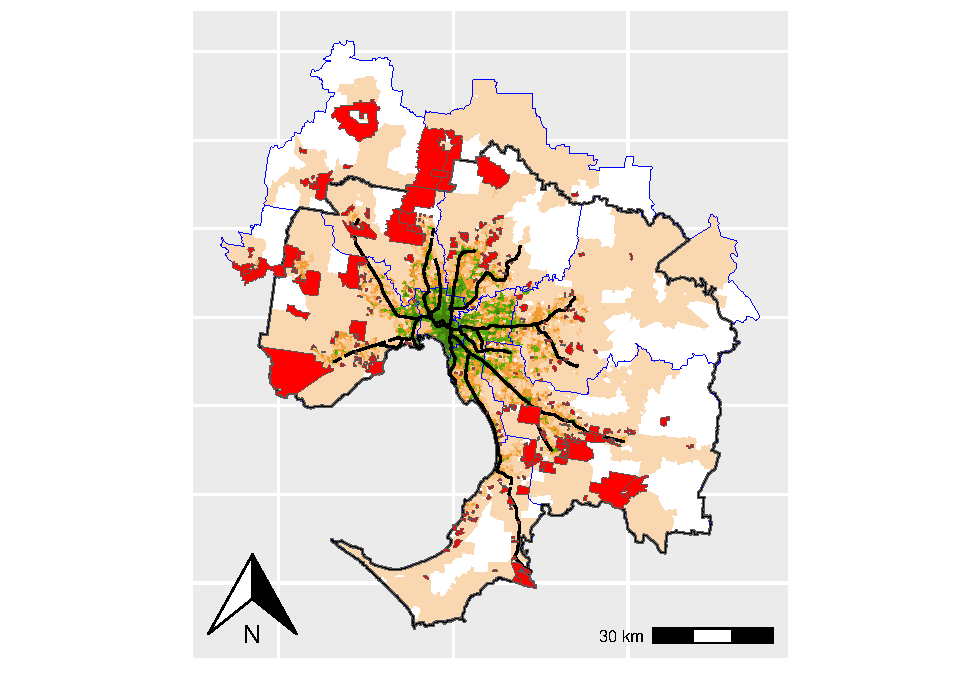
\includegraphics[width=1\linewidth]{Leveraging_GTFS_to_assess_transit_supply_Transport_Geography_files/figure-latex/Greater_Melbourne_2016_needs_gap_map_figure-1} \caption{Greater Melbourne 2016 SI groupings, overlayed with SA1s with very high transport need areas with zero or very low public transport supply (red).}\label{fig:Greater_Melbourne_2016_needs_gap_map_figure}
\end{figure}

\begin{figure}
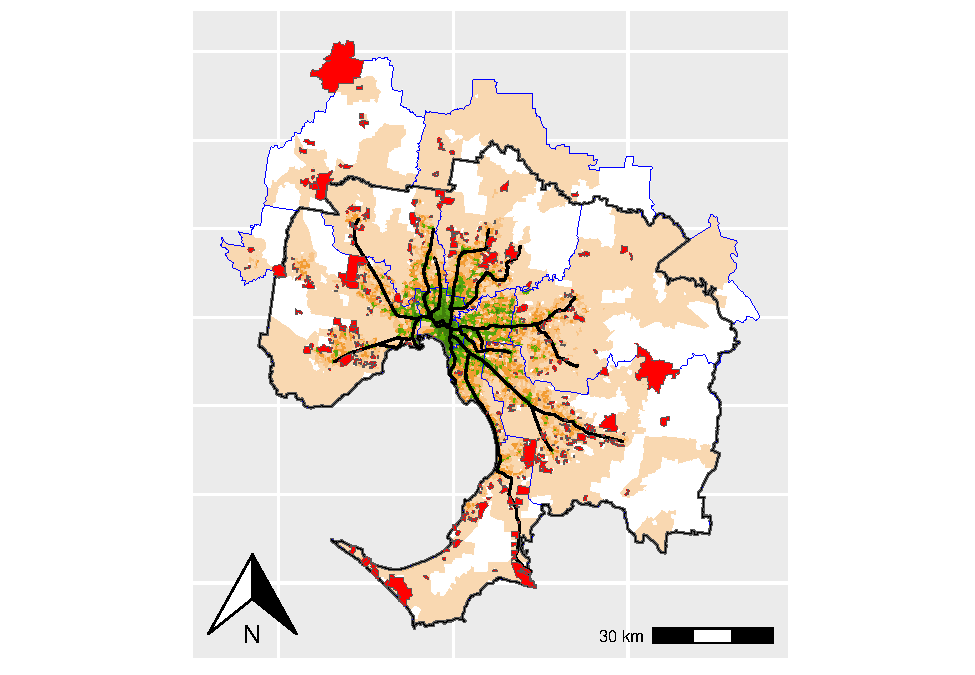
\includegraphics[width=1\linewidth]{Leveraging_GTFS_to_assess_transit_supply_Transport_Geography_files/figure-latex/Greater_Melbourne_2021_needs_gap_map_figure-1} \caption{Greater Melbourne 2021 SI groupings, overlayed with SA1s with very high transport need areas with zero or very low public transport supply (red).}\label{fig:Greater_Melbourne_2021_needs_gap_map_figure}
\end{figure}

Figures \ref{fig:Greater_Melbourne_2016_needs_gap_map_figure} and
\ref{fig:Greater_Melbourne_2021_needs_gap_map_figure} show SA1 zones in
Greater Melbourne with Very High transport needs, but Very Low or Zero
transit supply for 2016 and 2021. Comparison to the 2006 spatial
distribution shown in Figure \ref{fig:Currie_map_combined1}(bottom)
suggests that areas with large gaps between social needs and transit
supply continue to be mostly in the outer areas of Melbourne.
Comparisons of 2006 with 2016 and 2021 appear complicated by the larger
number of SA1s than CCDs, meaning that the maps in Figures
\ref{fig:Greater_Melbourne_2016_needs_gap_map_figure} and
\ref{fig:Greater_Melbourne_2021_needs_gap_map_figure} appear to show
more (smaller) areas with Very High transport needs, but Very Low or
Zero transit supply, including in the West, North West, North East and
South East parts of Greater Melbourne. The bottom parts of the Morning
Peninsula (around Blairgowrie) drop out of the category of having the
largest needs-gaps between 2006 and 2016, but are back in this category
again in 2021.

-COMPARE POPULATION WITH VERY HIGH NEEDS AND ZERO OR VERY LOW SUPPLY BY
SA4 between 2016 and 2021? - CROSSTAB THE 2021 HIGH GAPS WITH CHANGES IN
TRANSIT LEVEL?

\hypertarget{discussion}{%
\section{Discussion}\label{discussion}}

\hypertarget{limitations}{%
\subsection{Limitations}\label{limitations}}

\hypertarget{directions-for-furture-research}{%
\subsection{Directions for furture
research}\label{directions-for-furture-research}}

\hypertarget{conclusions}{%
\section{Conclusions}\label{conclusions}}

\hypertarget{references}{%
\section*{References}\label{references}}
\addcontentsline{toc}{section}{References}

\hypertarget{appendix}{%
\section{Appendix}\label{appendix}}

\begin{figure}
\centering
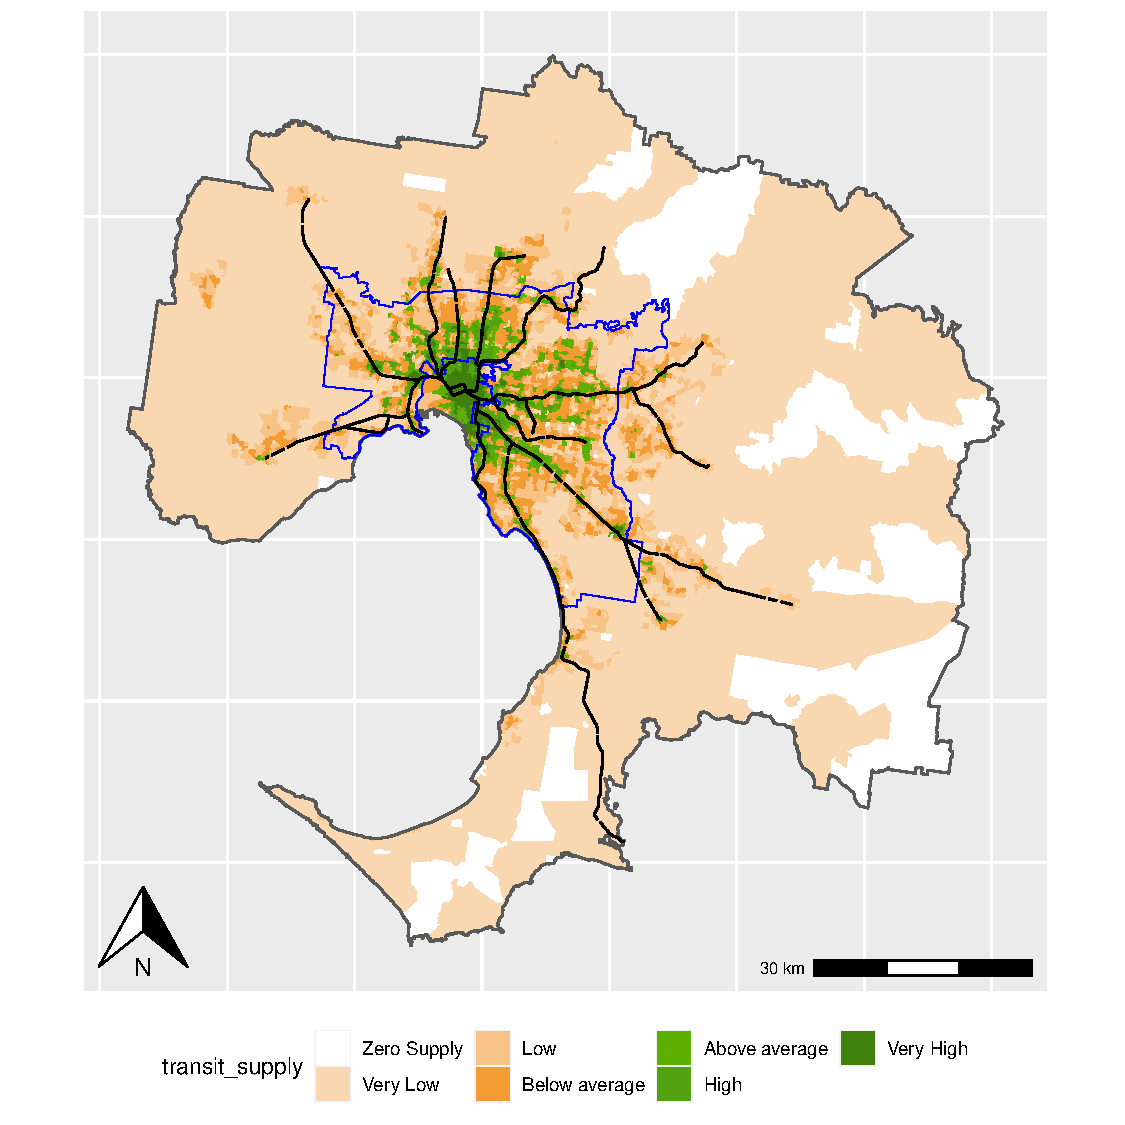
\includegraphics{Leveraging_GTFS_to_assess_transit_supply_Transport_Geography_files/figure-latex/Greater_Melbourne_CCD_2016_appendix-1.pdf}
\caption{Melbourne (2006 extents), Transport Supply by CCD, week
starting the day of the 2016 census, overlayed with inner/middle/outer
suburban boundary (blue) and suburban railway lines (black)}
\end{figure}

\begin{figure}
\centering
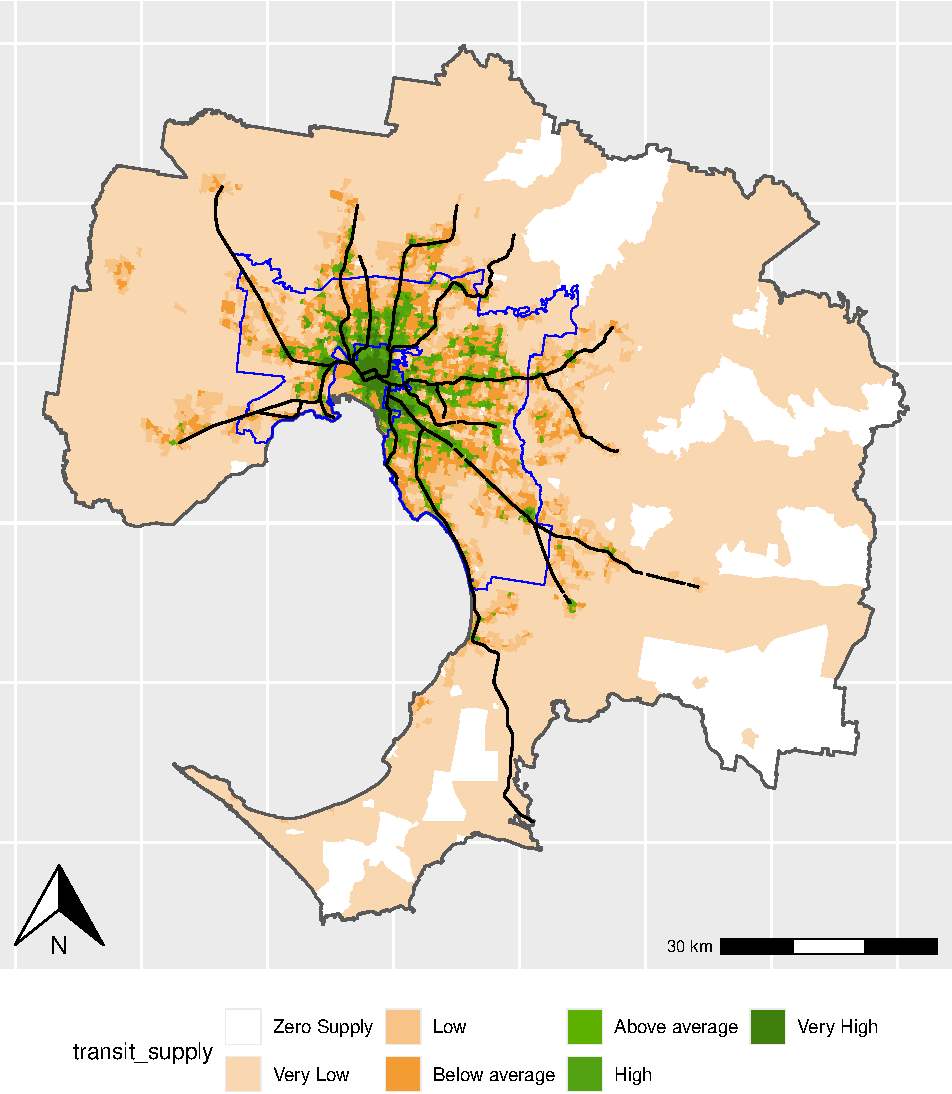
\includegraphics{Leveraging_GTFS_to_assess_transit_supply_Transport_Geography_files/figure-latex/Greater_Melbourne_CCD_2021_appendix-1.pdf}
\caption{Melbourne (2006 extents), Transport Supply by CCD, week
starting the day of the 2021 census, overlayed with inner/middle/outer
suburban boundary (blue) and suburban railway lines (black)}
\end{figure}

Figures \ref{fig:Greater_Melbourne_CCD_2016_appendix} and
\ref{fig:Greater_Melbourne_CCD_2021_appendix} show the distribution of
Transport Supply categories across Melbourne in the weeks of the 2016
censuses, using the same (2006) CCD boundaries\footnote{Note, however,
  that there are some inconsistencies in the CCDs included in
  Metropolitan Melbourne in \citet{currie2010identifying} (5,839) and
  the number included in ABS dataset used for this analysis (6,325).} as
in Figure \ref{fig:Currie_map_SI}. The overall spatial patterns appear
generally similar in 2016 and 2021 as they were in 2006, with higher
levels of transit supply in inner areas and close to most railway lines.
However, clear differences include:

\begin{itemize}
\tightlist
\item
  areas in the outer west (around Melton) that had above average supply
  in 2006 had below average supply in 2016 and 2021.
\item
  some middle south-eastern suburbs along the bay (in the vicinty of
  Black Rock) and outer eastern suburbs (Ferntree Gully) have dropped
  below average, while a small areas in the middle to outer south has
  moved from being below average in 2006 to above average in 2016
  (Kananook, immediately north of Frankston) and 2021 (Kananook and
  Bonbeach).
\item
  there have been suburban railway extensions to the north-west
  (Sunbury) and north-east (to South Morang in 2013 and to Mernda in
  2018). The former involved electrification to incorporate existing
  line segments (already served by country services) into the surburban
  network. Transport Supply to Sunbury, however, appears to still be
  below average, suggesting that not much has changed following the
  shift from service by regional trains to suburban trains. For Mernda
  in contrast, there has been increases in service levels, with some
  areas now having Above Average supply.
\item
  Some areas, away from railway lines, have also shifted from below
  average supply in 2006 to above average supplies in 2016 and 2021,
  including in the middle north-west (Greenvale) and middle to outer
  south east (Narre Warren South).
\item
  Services appear to have been introduced to some outer eastern (east of
  Gembrook), south-eastern (Koo Wee Rup, Lang Lang, Nar Nar Goon,
  Garfield, Bunyip and others) and southern (St Andrews Beach) areas.
\end{itemize}

\begin{figure}
\centering
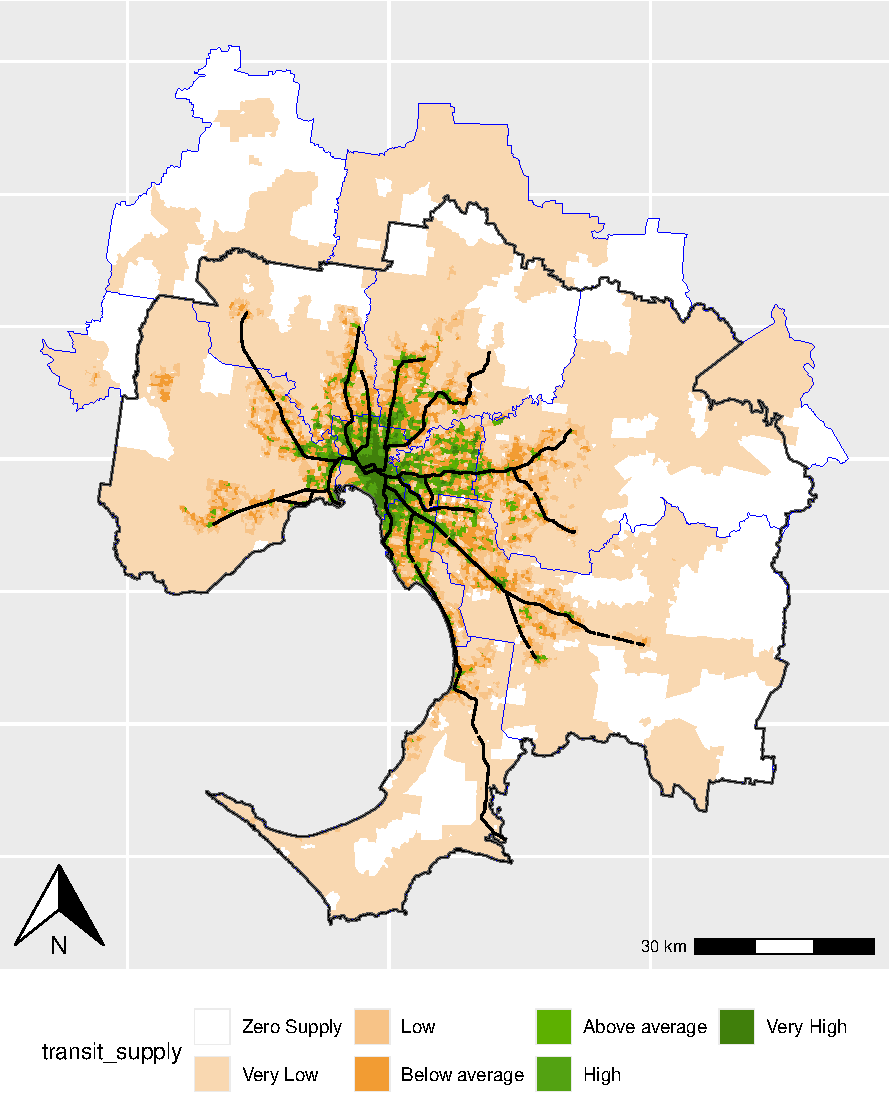
\includegraphics{Leveraging_GTFS_to_assess_transit_supply_Transport_Geography_files/figure-latex/Greater_Melbourne_SA12016_plot_appendix-1.pdf}
\caption{Greater Melbourne, Transit Supply by SA1 for the week starting
the date of the 2016 census, overlayed with: 2006 Greater Melbourne
boundary (black); 2021 SA4 boundaries (blue); and suburban railway lines
(black)}
\end{figure}

\begin{figure}
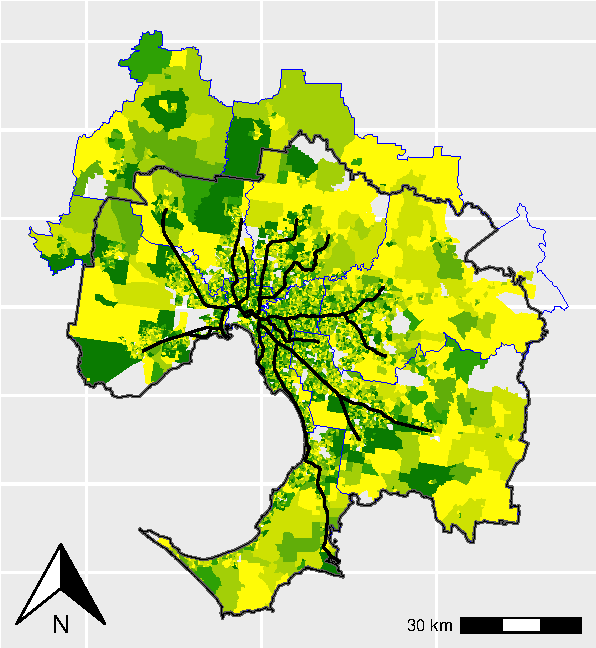
\includegraphics[width=0.9\linewidth]{Leveraging_GTFS_to_assess_transit_supply_Transport_Geography_files/figure-latex/Greater_Melbourne_2016_social_needs_appendix-1} \caption{Distribution of categories of composite social need index scores in 2016 (left) and 2021 (right), overlayed with: 2006 Greater Melbourne boundary (black); middle/outer and inner/middle suburb boundaries (grey); and suburban railway lines (dashed).}\label{fig:Greater_Melbourne_2016_social_needs_appendix}
\end{figure}

Figure \ref{fig:Greater_Melbourne_2016_social_needs_appendix} shows the
spatial patterns of social needs in 2016. Compared to 2021, the spatial
patterns appear similar, with some areas in the north-west (Gisborne)
and south-east (Carrum Downs, Stoney Point) having Very High needs in
both. Some caution may be required in making direct comparisons of many
outer suburbs where residential development has led to the introduction
of new SA1s for the 2021 census. In many areas, including in the
south-west (Werribee), north-west (Romsey), north (Wallan, Beveridge,
Mickleham) and south-east (Clyde North and Beaconsfield South), it
appears there are still Very High transport needs but the spatial area
covered on the map is much smaller due to the redistricting of larger
SA1s into multiple SA1s. That said, it appears that:

\begin{itemize}
\tightlist
\item
  social needs fell in the southern parts of Bacchus Marsh and areas
  around Melton (outer west);
\item
  social needs rose in some outer northern (Lancefield), eastern
  (Gembrook East) and southern (end of the Mornington Penninsula) areas.
\end{itemize}

\bibliography{References.bib, packages.bib}


\end{document}
